

	
	
	
	
	\chapter{Cadenas de algoritmos y Pipelines}\label{Cap6}
	
	%  Algorithm Chains and Pipelines
     \section{Introducción}
     
	Para muchos algoritmos de aprendizaje automático, la representación particular de los datos 
	que se proporcione es muy importante, como discutimos en el Capítulo \ref{Cap4}.  Esto comienza con el escalado de los datos y la combinación de características en forma manual  y  llega al extremo de aprendizaje de características  usando aprendizaje automático no supervisado, como vimos en el capítulo \ref{Cap3}.    En consecuencia, la mayoría las aplicaciones de aprendizaje automático requieren
	no sólamente la aplicación de un sólo algoritmo, sino de un encadenamiento de (o la unión)  muchos pasos diferentes de procesamiento y de modelos de aprendizaje automático.  En este capítulo, cubriremos cómo usar la clase {\ttfamily  Pipeline}  para simplificar proceso de construcción de cadenas de transformaciones y modelos. En particular, veremos cómo podemos combinar {\ttfamily Pipeline} y   {\ttfamily GridSearchCV} para buscar parámetros  con  todos los pasos de procesamiento a la vez.\\
	
	
	Como ejemplo de la importancia de encadenar modelos, observemos  como podemos 
	mejorar el rendimiento de un kernel SVM  sobre la dataset  de cáncer mediante el uso de {\ttfamily MinMaxScaler}  para preprocesamiento.   Aquí hay un código para dividir los datos, computando el mínimo y el  máximo, escalando la data y entrenando el SVM:
	
	
	\begin{lstlisting}%[frame=single]
	
In[1]:
	
   from sklearn.svm import SVC
   from sklearn.datasets import load_breast_cancer
   from sklearn.model_selection import train_test_split
   from sklearn.preprocessing import MinMaxScaler
	
   # load and split the data
   cancer = load_breast_cancer()
   X_train, X_test, y_train, y_test = train_test_split(
        cancer.data, cancer.target, random_state=0)
	
   # compute minimum and maximum on the training data
   scaler = MinMaxScaler().fit(X_train)
	
In[2]:
	
   # rescale the training data
   X_train_scaled = scaler.transform(X_train)
   
   svm = SVC()
   # learn an SVM on the scaled training data
   svm.fit(X_train_scaled, y_train)
   # scale the test data and score the scaled data
   X_test_scaled = scaler.transform(X_test)
   print("Test score: {:.2f}".format(
          svm.score(X_test_scaled, y_test)))
   
Out[2]:
   
   Test score: 0.95      
   \end{lstlisting}      
   
   \section{Selección de parámetros con preprocesamiento}
   
   
   Ahora supongamos que queremos encontrar los mejores parámetros para SVC usando {\ttfamily GridSearchCV}, como se discutió en el Capítulo \ref{Cap5}.  ¿Cómo deberíamos hacer esto?   Un enfoque ingenuo podría parecerse a esto:
   
   \begin{lstlisting}%[frame=single]
   
In[3]:
   
   from sklearn.model_selection import GridSearchCV
   # for illustration purposes only, don't use this code!
   param_grid = {'C': [0.001, 0.01, 0.1, 1, 10, 100],
   'gamma': [0.001, 0.01, 0.1, 1, 10, 100]}
   grid = GridSearchCV(SVC(), param_grid=param_grid, cv=5)
   grid.fit(X_train_scaled, y_train)
   print("Best cross-validation accuracy: {:.2f}".format(grid.best_score_))
   print("Best set score: {:.2f}".format(grid.score(X_test_scaled, y_test)))
   print("Best parameters: ", grid.best_params_)
   
Out[3]:
   
   Best cross-validation accuracy: 0.98
   Best set score: 0.97
   Best parameters: {'gamma': 1, 'C': 1}
   
   \end{lstlisting}
   
 
   
   Aquí, ejecutamos la búsqueda de cuadrícula (grid search) sobre los parámetros de SVC utilizando los datos escalados. Sin embargo,  hay una captura sutil en lo que acabamos de hacer.  Al escalar la data, usamos todos los datos del conjunto de entrenamiento para entrenarl el modelo. Luego usamos los datos de entrenamiento escalados  para correr búsqueda de cuadrícula (grid search)  usando validación cruzada. 
   Para cada división en la validación cruzada,  una parte de la data de entrenamiento original se declarará parte del entrenamiento de la división, y  otra parte  como  prueba de la división. La parte de prueba se utiliza para medir con datos nuevos el  modelo entrenado en la parte de entrenamiento. 
   Sin embargo, ya usamos la información contenida en la parte de prueba de la división, al escalar los datos.   Recuerda que  la parte de la prueba en cada división en la validación cruzada es parte del conjunto de entrenamiento, y  usamos la información de todo el conjunto de entrenamiento para encontrar la escala correcta de los datos.\\

   Esto   es fundamentalmente   diferente  de cómo los nuevos datos se ven para el  modelo.
   Si observamos la  nueva data (Digamos, en forma del conjunto de pruebas), estos datos no se habrán usado para escalar la data de entrenamiento, y podría tener un mínimo y un máximo  diferentes a los datos de entrenamiento.  El siguiente ejemplo (Figura \ref{Pipe1} ) muestra cómo es el procesamiento de datos durante la validación cruzada y la evaluación final:
   
\begin{lstlisting}%[frame=single]
   
In[4]:
   
   mglearn.plots.plot_improper_processing()
   
\end{lstlisting}
   
   
   \begin{figure}[h!]
      \centering
      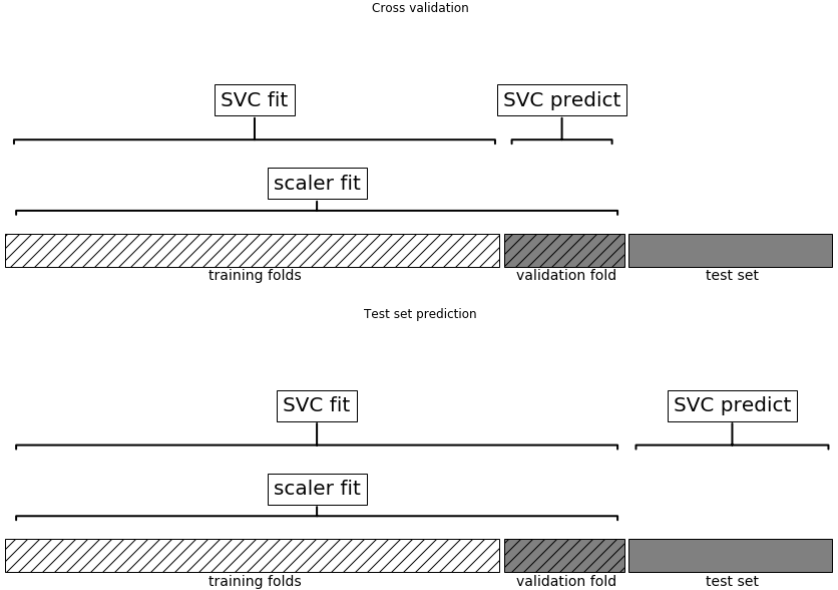
\includegraphics[scale=0.55]{Imagen_Machine/Pipe1.png}
      \caption{Uso de datos al preprocesar fuera del ciclo (Bucle) de validación cruzada}
      \label{Pipe1}
   \end{figure}
   
   
   Por lo tanto, las divisiones en la validación cruzada ya no reflejan correctamente cómo 
   se verán los nuevos datos en el proceso de modelado. Ya filtramos información de estas partes de la data en el proceso de modelado.  Esto conducirá a resultados demasiado optimistas durante
   validación cruzada, y posiblemente la selección de parámetros subóptimos.\\
   
   
   Para evitar este problema, la división del conjunto de datos durante la validación cruzada debe hacerse antes de hacer cualquier preprocesamiento. Cualquier proceso que extraiga conocimiento del conjunto de datos sólo debe aplicarse a la parte de la data de entrenamiento, por lo que cualquier validación cruzada debe ser el fuera del "{}bucle"{} en su procesamiento.\\

   En {\ttfamily scikit-learn} se lograr esto  con las funciones {\ttfamily cross\_val\_score} y    {\ttfamily Grid SearchCV}, mediante el uso de la clase {\ttfamily  Pipeline}. La clase {\ttfamily  Pipeline} es una clase que permite "{}pegar"{}  múltiples pasos de procesamiento en un sólo estimador de {\ttfamily scikit-learn}.
   La clase Pipeline tiene métodos de ajuste, predicción y métodos de  puntuación,  y se comporta como cualquier otro modelo en {\ttfamily scikit-learn}. El caso de uso más común de la clase {\ttfamily  Pipeline} es encadenar pasos de preprocesamiento (como escalar los datos) junto con un modelo supervisado como un clasificador.
   

   
   \subsection{Construyendo  Pipelines}
   
   Veamos cómo podemos usar la clase {\ttfamily  Pipeline} para expresar el flujo de trabajo para entrenar un modelo SVM después de escalar los datos con {\ttfamily MinMaxScaler} (por ahora sin  grid search). Primero, construimos un objeto  {\ttfamily  Pipeline} proporcionándole una lista de pasos. Cada paso es una tupla que contiene un nombre (cualquier cadena de su elección\footnote{Con una excepción: el nombre no puede contener un doble guión bajo, \_\_.}) y una instancia de un estimador:
   
   
\begin{lstlisting}%[frame=single]
   
In[5]:
   
   from sklearn.pipeline import Pipeline
   pipe = Pipeline([("scaler", MinMaxScaler()), ("svm", SVC())])
   
\end{lstlisting}
   

   Aquí, creamos dos pasos: el primero paso es el  llamado  de  "{}scaler"{}, es una instancia de {\ttfamily  MinMaxScaler}, y el segundo es  el llamado del modelo  "{}svm"{}, es una instancia de SVC. Ahora, podemos ajustar la {\ttfamily  Pipeline}, como cualquier otro estimador {\ttfamily scikit-learn}:
   
   \begin{lstlisting}%[frame=single]
      
In[6]:
   
   pipe.fit(X_train, y_train)   
   \end{lstlisting}  
   
   Aquí {\ttfamily pipe.fit},  el primer paso se llama el {\ttfamily fit} y hace el escalado de la data,  transforma la data de entrenamiento usando la escala definida, y finalmente se ajusta el modelo  SVM con la data escalada. Para evaluar sobre la data de prueba, simplemente llamamos a {\ttfamily pipe.score}:
   
   
   \begin{lstlisting}%[frame=single]
   
In[7]:
   
   print("Test score: {:.2f}".format(pipe.score(X_test, y_test)))
   
Out[7]:
   
   Test score: 0.95      
   \end{lstlisting}
   
   
   Llamando al método de puntuación sobre   pipeline,  primero transforma los datos de prueba usando la
   escala, y luego llama al método de puntuación sobre  el SVM usando la data de prueba escalada.
   Como  puede ver, el resultado es idéntico al que obtuvimos con el código al comienzo del
   capítulo, al hacer las transformaciones a mano.   Usando   pipeline, reducimos el
   código necesario para el proceso de "{}preprocesamiento {\scriptsize +}clasificación"{}. 
   Sin embargo, el principal beneficio de  usar  pipeline,  es que ahora podemos usar este estimador único en
   {\ttfamily cross\_val\_score} o   {\ttfamily GridSearchCV}.
   
   
   
   
   \subsection{Usando Pipelines en búsquedas de cuadrícula \\(Grid Searches)}
   
   Usando una pipeline con una búsqueda de cuadrícula  (grid search) funciona de la misma manera que usar cualquier otro estimador. Se define una la cuadrícula de parámetros,   y se construye un {\ttfamily GridSearchCV}  desde  la pipeline y la cuadrícula de parámetros. 
   
   Al especificar  la cuadrícula de parámetros, hay un ligero cambio; sin embargo,  necesitamos especificar para cada parámetro a qué paso del pipeline pertenece.   Ambos parámetros que queremos ajustar, {\ttfamily C  } y  {\ttfamily gamma}, son parámetros de SVC, el segundo paso. Le dimos a este paso el nombre  {\ttfamily  "{}svm"{}.}
   
   
   La sintaxis para definir una cuadrícula de parámetros en una pipeline  es para especificar por  cada parámetro el nombre del paso, seguido por un {\bf  \_\!\_} (un doble guión bajo), y  nombre del parámetro seguido.   De esta forma para buscar sobre el parámetro C  de SVC, tenemos que usar  {\ttfamily "{}svm{\bf \_\!\_}C"{} } como clave en el diccionario de cuadrícula de parámetros, y de manera similar para {\ttfamily gamma}:   
   
   \begin{lstlisting}   
   
In[8]:
   
   param_grid = {'svm__C': [0.001, 0.01, 0.1, 1, 10, 100],
                 'svm__gamma': [0.001, 0.01, 0.1, 1, 10, 100]} 
   \end{lstlisting}
   
   Con esta cuadrícula de parámetros podemos usar {\ttfamily GridSearchCV} como de costumbre:
     
        
   \begin{lstlisting}   
   
In[9]:
   
   grid = GridSearchCV(pipe, param_grid=param_grid, cv=5)
   grid.fit(X_train, y_train)
   print("Best cross-validation accuracy: {:.2f}".format(grid.best_score_))
   print("Test set score: {:.2f}".format(grid.score(X_test, y_test)))
   print("Best parameters: {}".format(grid.best_params_))
   
Out[9]:
   
   Best cross-validation accuracy: 0.98
   Test set score: 0.97
   Best parameters: {'svm__C': 1, 'svm__gamma': 1}   
   \end{lstlisting}
   
   En contraste con la búsqueda de cuadrícula que hicimos antes, ahora por  cada división en la validación cruzada, el {\ttfamily MinMaxScaler} es reacondicionado reajustado con sólo las divisiones del entrenamiento y no se filtra información de la división de prueba en la búsqueda de parámetros. 
   
   Esto se compara  (Figura \ref{Pipe2}) con la Figura {Pipe1} anterior en este capítulo:   
   
   \begin{lstlisting}
   
In[10]:
   
   mglearn.plots.plot_proper_processing()
   
   \end{lstlisting}
   
   \begin{figure}[h!]
      \centering
      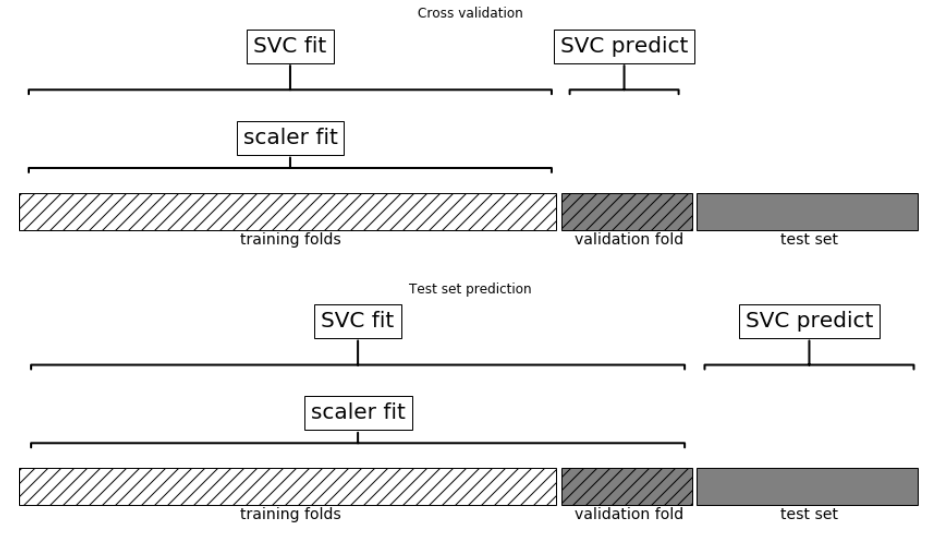
\includegraphics[scale=0.55]{Imagen_Machine/Pipe2}
      \caption{Uso de datos al preprocesamiento dentro del bucle de validación cruzada con una pipeline}
      \label{Pipe2}
   \end{figure}
   
     
   El impacto del filtrado de la información en la validación cruzada varía dependiendo de la naturaleza del paso de preprocesamiento. Estimar la escala de los datos usando el fold  de prueba por lo general no tiene un impacto terrible, mientras que el usando el fold de prueba en la extracción de características y la selección de características puede conducir a diferencias sustanciales en los resultados.
   
   
   
   
   
   
   %%%%%%%%%%%%%%%%%%%%%%%%%%%%%%%%    Caja     %%%%%%%%%%%%%%%%%%%%%%%%%%%%%%%%%%%%%%%%%
   
   
   
   
   
   
   
   \begin{longtable}{|p{13.25cm}|}  
      
      
      \arrayrulecolor{red}\hline
      
      \begin{center}
         {\bf{Ilustrando la filtración de información}}
      \end{center}
      
      \endfirsthead
      %   \hline
      
      Un gran ejemplo de información filtrada en validación cruzada se da en  el libro  The Elements of Statistical Learning  de  Friedman’s  de  Hastie,   Tibshirani,  aquí reproducimos una versión adaptada.    Consideremos una tarea de regresión sintética con 100 muestras y 10.000 características
		que se muestrean independientemente de una distribución gaussiana. También se muestrea
		la respuesta de una distribución gaussiana:       \\
		
		%	\endhead
		
		{ \ttfamily   
			{\scriptsize{  	
					
	            In[11]:
               \vspace{0.1cm}
               
     
   
            {\color{blue}   {\textbf
          {\hspace{0.6cm}from  rnd = np.random.RandomState(seed={\color{red} 0})}
                     
           \hspace{0.6cm}X = rnd.normal(size=({\color{red}  100 }, {\color{red}  10000})    \vspace{-0.2cm} 
                     
           \hspace{0.6cm}y = rnd.normal(size=({\color{red} 100},))  
      }  }}}}\\       
      
      \vspace{-0.251cm}
      
      
      Dada la forma en que creamos la dataset, no hay relación entre los datos   X,  y  el
      objetivo $y$ (target)  (es decir, son independientes), por lo que no debería ser posible aprender nada de  esta  dataset. Ahora haremos lo siguiente. Primero, seleccionemos las  características  más informativas de los 10,   usando para la selección de características {\ttfamily SelectPercentile}, y
   	luego evaluamos al regresor Ridge   utilizando validación cruzada: \\  
		
		
		{ \ttfamily   
			{\scriptsize{  	
					
					In[12]:
					\vspace{0.1cm}
					
				\hspace{0.6cm}{\color{blue} {\textbf   from  sklearn.feature\_selection import SelectPercentile, f\_regression
							
				\hspace{0.6cm}select = SelectPercentile(score\_func=f\_regression, percentile=  {\color{red} 5}).fit(X, y)
							
				\hspace{0.6cm}X\_selected = select.transform(X)  
							
				\hspace{0.6cm}print({\color{red}  "{}X\_selected.shape: "{}}.format(X\_selected.shape))   }}
					\vspace{0.1cm}
					
					Out[12]:
					\vspace{0.1cm}
					
					\hspace{0.6cm}X\_selected.shape: (100, 500)
					\vspace{0.1cm}
					
					In[13]:
					\vspace{0.1cm}
					
				\hspace{0.6cm}{\color{blue}	{\textbf from  sklearn.model\_selection import cross\_val\_score
							
				\hspace{0.6cm}from sklearn.linear\_model import Ridge
							
				\hspace{0.6cm}print({\color{red}  "{}Cross-validation accuracy (cv only on ridge): {:.2f}"{}}.format(
							
				\hspace{1.65cm}np.mean(cross\_val\_score(Ridge(), X\_selected, y, cv={\color{red} 5}))))
					}}
					\vspace{0.1cm}
					
					Out[13]:
					\vspace{0.1cm}
					
			\hspace{0.6cm}Cross-validation accuracy (cv only on ridge): 0.91 }}}	\\
		
		\vspace{-0.251cm}
		
		
		La promedio  de  $R^{2}$  calculada  por validación cruzada es  0.91,  lo que indica un modelo muy bueno. 
		Esto claramente no puede ser correcto, ya que los datos son completamente aleatorios. 
		Lo que sucedió aquí es que nuestra selección de características escogió algunas características
		entre las 10.000 características aleatorias que están (por casualidad) muy bien correlacionadas
		con el objetivo. Debido a que ajustamos la selección de características fuera de la 
		validación cruzada, podría 		encontrar características que están correlacionadas tanto en el entrenamiento como en los folds  		 de prueba. 
		La información que filtramos de los folds  de prueba fue muy informativa, lo que 
		llevó a resultados muy poco realistas. Comparemos esto con una validación cruzada apropiada
		usando una pipeline:\\
		
		
		{ \ttfamily   
			{\scriptsize{  	
					
					In[14]:
					\vspace{0.1cm}
					
				\hspace{0.6cm}{\color{blue} {\textbf   pipe = Pipeline([("{}select"{}, SelectPercentile(score\_func=f\_regression,
							
			\hspace{3.4cm}percentile=5)), ("{}ridge"{}, Ridge())])
							
			\hspace{0.6cm}print("{}Cross-validation accuracy (pipeline): {:.2f}"{}.format(
							
			\hspace{1.65cm}np.mean(cross\_val\_score(pipe, X, y, cv=5))))  } }
					\vspace{0.1cm}
					
					Out[14]:
					\vspace{0.1cm}
					
			\hspace{0.6cm}Cross-validation accuracy (pipeline): -0.25  }}}	\\
		
		\vspace{-0.251cm}
		
		
		Esta vez, obtenemos una puntuación $R^{2}$  negativa, indicando un modelo muy pobre.
		Utilizando la pipeline, la selección de características se encuentra ahora dentro del bucle 
		de validación cruzada. Esto significa que las características sólo se pueden seleccionar 
		utilizando los folds  de la data de entrenamiento, no el folds de prueba. 
		La selección de características encuentra las características que están correlacionadas
		con el objetivo en el conjunto de entrenamiento, pero debido a que los datos son 
		completamente aleatorios, estas características no están correlacionadas con el objetivo 
		en el conjunto de pruebas. En este ejemplo, rectificar el problema de la filtración de la 
		data en la selección  característica hace la diferencia entre la conclusión de que un modelo
		funciona muy bien y la conclusión de que un modelo no funciona en absoluto. \\
		% \vspace{0.1cm}
		\\  	
		\arrayrulecolor{red}\hline
		
	\end{longtable}
	

	
	\section{Interfaz general  de  Pipeline}
	
	La clase Pipeline no está restringida al preprocesamiento y clasificación, sino que puede
	unir cualquier cantidad de estimadores. Por ejemplo, podría construir una  pipeline
	que contiene la extracción de características, selección de características, escalado y clasificación, para un total de cuatro pasos. Del mismo modo, el último paso podría ser la regresión o clúster en lugar de la clasificación.  El único requisito para los estimadores en una pipeline es que todos, excepto el último paso, necesitan tener un método de transformación, para que puedan producir una nueva representación de los datos que se puede usar en el siguiente paso.\\
	
	
	Internamente, durante el  llamado a {\ttfamily Pipeline.fit},  pipeline llama {\ttfamily fit }  y luego   {\ttfamily  transform}  en cada paso por turno\footnote{O simplemente {\ttfamily fit\_transform}}, con la entrada dada por la salida del método de {\ttfamily  transform} del paso anterior. 
	Para el último paso en pipeline, sólo se llama {\ttfamily fit}.\\
	
	
	%    Brushing   raspando   Repasando algunos detalles más finos,
	%    Brushing over some finer details, this is implemented as follows. %
	
	Al dejar algunos detalles más finos, esto se implementa de la siguiente manera.
	Recuerda que {\ttfamily pipeline.steps} es una lista de tuplas, por lo que {\ttfamily pipeline.steps[0][1] }  es el primer estimador, {\ttfamily pipeline.steps[1][1]} es el segundo estimador, y así sucesivamente:
	
	
	\begin{lstlisting}%[frame=single]
	
In[15]:
   
   def fit(self, X, y):
       X_transformed = X
       for name, estimator in self.steps[:-1]:
           # iterate over all but the final step
           # fit and transform the data
           X_transformed = estimator.fit_transform(X_transformed, y)
       # fit the last step
       self.steps[-1][1].fit(X_transformed, y)
       return self   
   \end{lstlisting}
   

   Al predecir usando  {\ttfamily Pipeline}, transformamos de manera similar los datos con  {\ttfamily transform},   usando todo menos el último paso, y luego llamamos a predecir con  {\ttfamily predict} en el último paso:
   
   \begin{lstlisting}%[frame=single]
   
In[16]:
   
   def predict(self, X):
       X_transformed = X   
       for step in self.steps[:-1]:
           # iterate over all but the final step
           # transform the data
           X_transformed = step[1].transform(X_transformed)
       # fit the last step
       return self.steps[-1][1].predict(X_transformed)	
	\end{lstlisting}
	
	
	
	El proceso se ilustra en la figura \ref{Pipe3} para dos transformadores, T1,  T2, y un clasificador (llamado  {\ttfamily Classifier} ).
	
	\begin{figure}[h!]
		\centering
		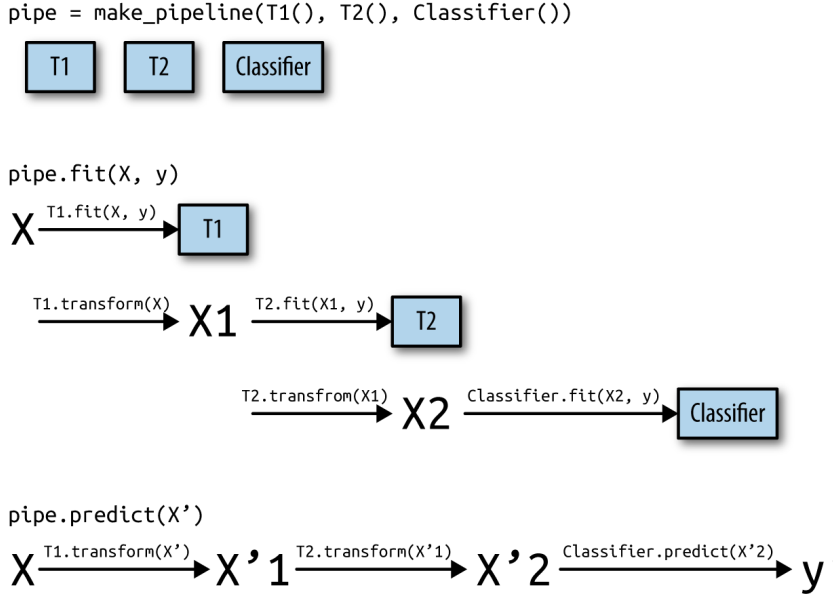
\includegraphics[scale=0.65]{Imagen_Machine/Pipe3}
		\caption{Descripción general del proceso de entrenamiento y predicción de pipeline}
		\label{Pipe3}
	\end{figure}
	
	
	La pipeline es incluso más general que esto. No es necesario que el último paso en un pipeline para 
	tener  una función de predicción, y podríamos crear una pipeline que sólo contenga, por ejemplo, un escalador y un PCA. Entonces, debido a que el último paso (PCA) tiene un método de transformación, podríamos llamar a {\ttfamily transform} en la pipeline  para obtener la salida de {\ttfamily  PCA.transform} aplicada a los datos que se procesaron en el paso anterior. El último paso de una pipeline sólo se requiere  tener un método {\ttfamily fit}.
	
	\newpage
	
	\subsection{Creando  una  Pipeline   con  {\ttfamily make\_pipeline}}

     	%  cumbersome  =    engorroso
	
	Crear una pipeline  usando la sintaxis descrita anteriormente es algunas veces un poco engorroso, y a menudo no necesitamos usar nombres especificos por cada paso. Hay una función de conveniencia, {\ttfamily make\_pipeline}, que creará una pipeline personal y nombrará automáticamente cada paso basado en su clase. La sintaxis para {\ttfamily make\_pipeline}, es la siguiente:
	
	
	
	\begin{lstlisting}%[frame=single]
	
In[17]:
	
   from sklearn.pipeline import make_pipeline
   # standard syntax
   pipe_long = Pipeline([("scaler", MinMaxScaler()), ("svm", SVC(C=100))])
   # abbreviated syntax
   pipe_short = make_pipeline(MinMaxScaler(), SVC(C=100))   
   \end{lstlisting}
   
   
   Los objetos pipeline son {\ttfamily pipe\_long}  y  {\ttfamily pipe\_short}  hacen exactamente lo mismo, pero {\ttfamily pipe\_short} tiene pasos que se nombran automáticamente. Podemos ver los nombres de los pasos observando el atributo {\ttfamily steps}:
   
   
   \begin{lstlisting}%[frame=single]
   
   
In[18]:
   
   print("Pipeline steps:\n{}".format(pipe_short.steps))
   
Out[18]:
   
   Pipeline steps:
   [('minmaxscaler', MinMaxScaler(copy=True, feature_range=(0, 1))),
    ('svc', SVC(C=100, cache_size=200, class_weight=None, coef0=0.0,
                decision_function_shape=None, degree=3, gamma='auto',
                kernel='rbf', max_iter=-1, probability=False,
                random_state=None, shrinking=True, tol=0.001,
                verbose=False))]   
   \end{lstlisting}
   
   	
	Los pasos se llaman {\ttfamily minmaxscaler}  y  {\ttfamily svc}. En general, los nombres de los pasos 
	son sólo versiones minúsculas de los nombres de clase. Si varios pasos tienen la misma clase,
	se añade un número:
	
	\begin{lstlisting}%[frame=single]
   
In[19]:
   
   from sklearn.preprocessing import StandardScaler
   from sklearn.decomposition import PCA
   
   pipe = make_pipeline(StandardScaler(), PCA(n_components=2), 
                        StandardScaler())
   print("Pipeline steps:\n{}".format(pipe.steps))
   
Out[19]:
   
   Pipeline steps:
   [('standardscaler-1', StandardScaler(copy=True, with_mean=True,
                                        with_std=True)), 
    ('pca', PCA(copy=True, iterated_power=4, n_components=2, 
                random_state=None, svd_solver='auto', tol=0.0,
                whiten=False)), 
    ('standardscaler-2', StandardScaler(copy=True, with_mean=True, 
                                         with_std=True))]   
   \end{lstlisting}
  	
	Como puedes ver, el primer paso {\ttfamily StandardScaler} fue nombrado como  {\ttfamily standardscaler-1} y el segundo paso lo nombra como {\ttfamily standardscaler-1}. Sin embargo, en tales escenarios podría ser mejor usar la construcción del {\ttfamily Pipeline} con nombres explícitos, para dar nombres relacionados con cada paso.
	
	\subsection{Acceso a los atributos por pasos}
	
	
	Es posible que se necesite inspeccionar los atributos en uno de los pasos de la pipeline, por ejemplo, los coeficientes de un modelo lineal o los componentes extraídos por PCA. La forma más fácil de acceder a los pasos en una pipeline es a través del atributo {\ttfamily named\_steps}, que es un diccionario de los nombres de los pasos en los estimadores:	
	
	
	\begin{lstlisting}%[frame=single]
	
In[20]:
	
   # fit the pipeline defined before to the cancer dataset
   pipe.fit(cancer.data)
   # extract the first two principal components from the "pca" step
   components = pipe.named_steps["pca"].components_
   print("components.shape: {}".format(components.shape))
   
Out[20]:
   
    components.shape: (2, 30)   
	\end{lstlisting}
	
	
	
	\subsection{Acceso a atributos de una Pipeline dentro de una  buscada de cuadrícula}
	%   Grid-Searched 
	
	
	
	Como discutimos anteriormente en este capítulo, una de las principales razones para usar las
	pipelines  es para hacer búsquedas de cuadriculas (grid searches). Una tarea común es acceder 
	 a algunos de los pasos   de una pipelines dentro de una búsqueda  cuadrícula.
	Hagamos una Busqueda de cuadrícula en el clasificador   {\ttfamily LogisticRegression} sobre la dataset de cáncer, usando {\ttfamily Pipeline} y {\ttfamily StandardScaler} para 
	escalar los datos antes de pasarlos al clasificador  {\ttfamily LogisticRegression}.  Primero creamos una pipeline usando la función {\ttfamily make\_pipeline}: 
	
	
	\begin{lstlisting}%[frame=single]
	
In[21]:
	
   from sklearn.linear_model import LogisticRegression
   
   pipe = make_pipeline(StandardScaler(), LogisticRegression())   
   \end{lstlisting} 
	
	
	A continuación, creamos una cuadrícula de parámetros. Como se explicó en el capítulo \ref{Cap2}, 
	\: el parámetro de regularizaciónen  para ajustar en  {\ttfamily LogisticRegression}, es el parámetro C. Usamos una cuadrícula logarítmica para este parámetro, buscando entre 0.01 y 100. Debido a que usamos la función {\ttfamily make\_pipeline}, el nombre del paso {\ttfamily LogisticRegression } en la pipeline  es el nombre de clase en letras minúsculas, {\ttfamily logisticregression}.   Por lo tanto para ajustar el parámetro C, tenemos que especificar una cuadrícula de parámetros para {\ttfamily logisticregression{\scriptsize\_\!\_\!\_}C}:
	
	\begin{lstlisting}
	
In[22]:
	
   param_grid = {'logisticregression__C': [0.01, 0.1, 1, 10, 100]}
   
   \end{lstlisting}
   
   
   Como de costumbre, dividimos la dataset del cáncer en dos conjuntos, el de entrenamiento y el prueba, y ajustamos una búsqueda de cuadrícula:   
   
   \begin{lstlisting}
   
In[23]:
   
   X_train, X_test, y_train, y_test = train_test_split(
       cancer.data, cancer.target, random_state=4)
   grid = GridSearchCV(pipe, param_grid, cv=5)
   grid.fit(X_train, y_train)
   
   \end{lstlisting}
   
   Y ahora, ¿cómo accedemos a los coeficientes del mejor modelo de  clasificación {\ttfamily LogisticRegression}    encontrado por {\ttfamily  GridSearchCV} ?.    Del Capítulo \ref{Cap5} sabemos que el     mejor  modelo encontrado por  {\ttfamily  GridSearchCV}, entrenado en todos los datos de entrenamiento, es almacenado en {\ttfamily grid.best\_estimator\_}:
   
   
   \begin{lstlisting}%[frame=single]
   
In[24]:
   
   print("Best estimator:\n{}".format(grid.best_estimator_))
	
Out[24]:
   
   Best estimator:
   Pipeline(steps=[
       ('standardscaler', StandardScaler(copy=True, with_mean=True, 
         with_std=True)),
       ('logisticregression', LogisticRegression(C=0.1, class_weight=None,
         dual=False, fit_intercept=True, intercept_scaling=1, max_iter=100,
         multi_class='ovr', n_jobs=1, penalty='l2', random_state=None,
         solver='liblinear', tol=0.0001, verbose=0, warm_start=False))])   
   \end{lstlisting}
   En este caso se accede a los pasos con  {\ttfamily best\_estimator\_}. Ahora, en nuestro caso que es una pipeline con dos pasos, {\ttfamily
      standardscaler}  y  {\ttfamily logisticregression}, para acceder a los pasos  se  usar el atributo {\ttfamily  named\_steps} de la pipeline,   en   {\ttfamily logisticregression},  como se explicó anteriormente.
   
   \begin{lstlisting}%[frame=single]
   
In[25]:
   
   print("Logistic regression step:\n{}".format(
          grid.best_estimator_.named_steps["logisticregression"]))
   
Out[25]:
	
   Logistic regression step:
   LogisticRegression(C=0.1, class_weight=None, dual=False, 
                      fit_intercept=True, intercept_scaling=1,
                      max_iter=100, multi_class='ovr', n_jobs=1,
                      penalty='l2', random_state=None, 
                      solver='liblinear', tol=0.0001, verbose=0,
                      warm_start=False)
   
   \end{lstlisting}
   
	Ahora que hemos entrenado la instancia  {\ttfamily LogisticRegression}, podemos acceder a los coefficientes (o pesos) asociados con cada característica de entrada:	
	
	
	\begin{lstlisting}%[frame=single]
	
In[26]:
	
   print("Logistic regression coefficients:\n{}".format(
          grid.best_estimator_.named_steps["logisticregression"].coef_))
   
Out[26]:
   
   Logistic regression coefficients:
   [[-0.389 -0.375 -0.376 -0.396 -0.115 0.017 -0.355 -0.39 -0.058 0.209
   -0.495 -0.004 -0.371 -0.383 -0.045 0.198 0.004 -0.049 0.21 0.224
   -0.547 -0.525 -0.499 -0.515 -0.393 -0.123 -0.388 -0.417 -0.325 -0.139]]   
   \end{lstlisting}
   
   Esto puede ser una expresión algo larga, pero con frecuencia es útil  para entender los modelos.
   
   \subsection{Pasos en el preprocesamiento de búsqueda de cuadrícula y parámetros del modelo} 
	% Grid-Searching Preprocessing Steps and Model Parameters 
	
	Usando pipelines, podemos encapsular todos los pasos de procesamiento en el flujo de trabajo del aprendizaje automático en un sólo estimador de {\ttfamily  scikit-learn}.  	Otro beneficio de usar el pipelina, es que ahora podemos ajustar los parámetros del 
	preprocesamiento utilizando  el resultado de una tarea supervisada como la regresión
	o clasificación.
	
	En capítulos anteriores, utilizamos  algunas  características polinómicas en la dataset  boston antes de aplicar el regresor ridge. Ahora vamos a modelar esto  utilizando una pipeline. La pipeline contiene tres pasos:  escala la data,  cálculo las características polinómicas, y la regresión de ridge:
	
	
	
	\begin{lstlisting}%[frame=single]
	
In[27]:
	
   from sklearn.datasets import load_boston
   boston = load_boston()
   X_train, X_test, y_train, y_test = train_test_split(
        boston.data, boston.target, random_state=0)
   
   from sklearn.preprocessing import PolynomialFeatures
   pipe = make_pipeline( StandardScaler(),
                         PolynomialFeatures(),
                         Ridge())
   
   \end{lstlisting}
   
   
   
   ¿Cómo sabemos qué grados de polinomios elegir, o qué  polinomio   elegir o qué interacciones? Idealmente queremos seleccionar el parámetro de grado basado en el resultado de la clasificación.
	Usando nuestra   pipeline, podemos buscar sobre el parámetro  {\ttfamily degree} junto con el parámetro {\ttfamily alfa} de {\ttfamily  Ridge}. Para hacer esto, definimos el parámetro  {\ttfamily param\_grid} que contiene ambos, adecuadamente prefijado por los nombres del respectivo  paso: 
	
	
	\begin{lstlisting}%[frame=single]
	
In[28]:
	
    param_grid = {'polynomialfeatures__degree': [1, 2, 3],
                  'ridge__alpha': [0.001, 0.01, 0.1, 1, 10, 100]}   
   \end{lstlisting}
   
	
	
	
	Ahora podemos correr nuevamente la busqueda de cuadrícula:
	
	
	\begin{lstlisting}%[frame=single]
	
	
In[29]:
	
   grid = GridSearchCV(pipe, param_grid=param_grid, cv=5, n_jobs=-1)
   grid.fit(X_train, y_train)	
	\end{lstlisting}	
	
	
Podemos visualizar el resultado de la validación cruzada usando un mapa caliente  (Figura \ref{Pipe4}), como hicimos en el Capítulo \ref{Cap5}:
	
	
	\begin{lstlisting}%[frame=single]
	
In[30]:
	
   plt.matshow(grid.cv_results_['mean_test_score'].reshape(3, -1),
               vmin=0, cmap="viridis")
   plt.xlabel("ridge__alpha")
   plt.ylabel("polynomialfeatures__degree")
   plt.xticks(range(len(param_grid['ridge__alpha'])), 
              param_grid['ridge__alpha'])
   plt.yticks(range(len(param_grid['polynomialfeatures__degree'])),
              param_grid['polynomialfeatures__degree'])
   
   plt.colorbar()	
	\end{lstlisting}	

	
	\begin{figure}[h!]
		\centering
		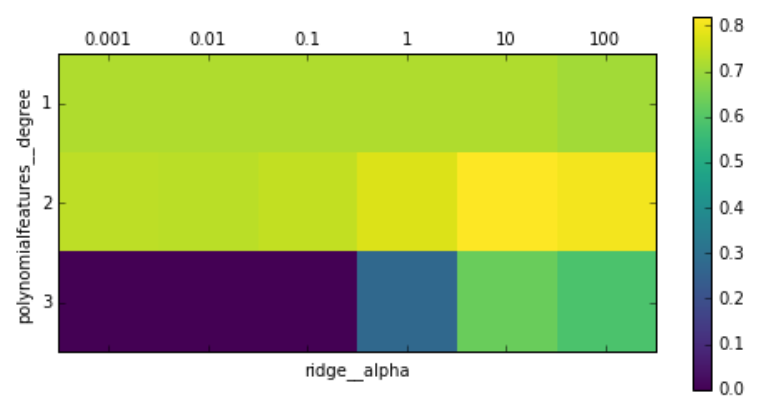
\includegraphics[scale=0.55]{Imagen_Machine/Pipe4}
		\caption{Mapa caliente del puntuación media de la validación cruzada como  función del grado de las características polinómicas y del parámetro {\ttfamily alfa} de  {\ttfamily  Ridge}}
		\label{Pipe4}
	\end{figure}
\newpage	
	Observando estos  resultados producidos por la validación cruzada, podemos ver que el uso 
	de polinomios de grado dos ayuda, pero que los polinomios de grado tres son mucho peores que cualquiera de los grados uno o dos. Esto se refleja en los mejores parámetros que se encontraron:
	
	
	\begin{lstlisting}%[frame=single]
	
In[31]:
	
   print("Best parameters: {}".format(grid.best_params_))
	
Out[31]:
	
   Best parameters: {'polynomialfeatures__degree': 2, 'ridge__alpha': 10}
	
	\end{lstlisting}
	
	Que conducen a la siguiente puntuación:
	
	
	
	\begin{lstlisting}%[frame=single]
	
In[32]:
	
   print("Test-set score: {:.2f}".format(grid.score(X_test, y_test)))
	
Out[32]:
	
   Test-set score: 0.77	
	\end{lstlisting}
	
	Vamos a ejecutar una búsqueda de cuadrícula sin características polinómicas para la comparación:
	
	
	
	\begin{lstlisting}%[frame=single]
	
In[33]:
	
   param_grid = {'ridge__alpha': [0.001, 0.01, 0.1, 1, 10, 100]}
   pipe = make_pipeline(StandardScaler(), Ridge())
   grid = GridSearchCV(pipe, param_grid, cv=5)
   grid.fit(X_train, y_train)
   print("Score without poly features: {:.2f}".format(
          grid.score(X_test, y_test)))
   
Out[33]:
   
	Score without poly features: 0.63
  \end{lstlisting}
 	
	
	Como se  esperaba, observando los resultados de búsqueda de cuadrícula visualizados en la figura \ref{Pipe4}, usando características no polinómicas conduce a resultados de puntajes más bajos, es decir, un modelo con rendimiento peor con respecto al anterior.\\
   %   ningún polinomio
	
	La búsqueda de parámetros de preprocesamiento junto con parámetros del modelo 
	es una estrategia muy poderosa. Sin embargo, tenga en cuenta que  {\ttfamily GridSearchCV }  
	intenta todas las combinaciones posibles de los parámetros especificados. Por lo tanto,
	agregar más parámetros a su cuadrícula aumenta exponencialmente el número de modelos que
	necesita construir.
	
	
	\subsubsection{Qué modelo utilizar y	Grid-Searching }
	
	%    Grid-Searching Which Model To Use

	
	Incluso puede ir más allá al combinar {\ttfamily GridSearchCV} y  {\ttfamily  Pipeline}: 
	también es posible  buscar  los pasos reales que se realizó la pipeline (ya sea usando {\ttfamily
		StandardScaler}  o   {\ttfamily MinMaxScaler}).
	Esto lleva a un espacio de búsqueda aún mayor y debe ser considerado cuidadosamente. Probar todas las soluciones posibles generalmente no es una estrategia viable de aprendizaje automático. 
	Sin embargo, aquí hay un ejemplo comparando un clasificador de {\ttfamily RandomForest}
	y uno de {\ttfamily  SVC} en la dataset Iris. Sabemos que el {\ttfamily  SVC} podría necesitar la dataset  escalar, por lo que también buscamos si se usa {\ttfamily  StandardScaler}  o no preprocesando.
	Para el {\ttfamily RandomForestClassifier}, sabemos que no es necesario ningún preprocesamiento.
	Comenzamos definiendo la pipeline; aquí, nombramos explícitamente los pasos. 
	Queremos dos pasos, uno para el preprocesamiento y el siguiente para un clasificador. Podemos instanciar esto 	usando {\ttfamily  SVC}  y  {\ttfamily  StandardScaler}:
		
	
	\begin{lstlisting}
	
In[34]:
   
   pipe = Pipeline([('preprocessing', StandardScaler()),
                    ('classifier', SVC())])   
   \end{lstlisting}
	
	%        “ busque sobre espacios que no son cuadrículas ”
	
	Ahora podemos definir el  {\ttfamily  parametr\_grid} para hacer la busqueda. Usaremos el clasificador  {\ttfamily RandomForestClassifier} o {\ttfamily SVC}. Ambos tienen diferentes parámetros para ajustar, por lo que  necesitan diferentes preprocesamientos, podemos hacer uso de la lista de  search grids  (búsqueda de cuadrículas)  que discutimos en "{}Buscar sobre espacios que no son cuadrículas"{}  en la página  \pageref{Pagina1}.
	
	
	Para asignarle  un estimador a un paso, usamos el nombre del paso como nombre del parámetro. Cuando necesitamos  saltar un paso en el pipeline (por ejemplo, porque no necesitamos preprocesamiento para {\ttfamily RandomForest}), no lo configuramos en ningún paso:	
	
	\begin{lstlisting}   
In[35]:
   
   from sklearn.ensemble import RandomForestClassifier
   
   param_grid = [
   {'classifier': [SVC()], 'preprocessing': [StandardScaler(), None],
   'classifier__gamma': [0.001, 0.01, 0.1, 1, 10, 100],
   'classifier__C': [0.001, 0.01, 0.1, 1, 10, 100]},
   {'classifier': [RandomForestClassifier(n_estimators=100)],
    'preprocessing': [None], 'classifier__max_features': [1, 2, 3]}]	
	\end{lstlisting}
	
Ahora podemos iniciar y ejecutar la búsqueda de cuadrícula como de costumbre, 
	en este caso sobre la data de cáncer:
	
	\begin{lstlisting}	
In[36]:
	
   X_train, X_test, y_train, y_test = train_test_split(
       cancer.data, cancer.target, random_state=0)
   
   grid = GridSearchCV(pipe, param_grid, cv=5)
   grid.fit(X_train, y_train)
   
   print("Best params:\n{}\n".format(grid.best_params_))
   print("Best cross-validation score: {:.2f}".format(grid.best_score_))
   print("Test-set score: {:.2f}".format(grid.score(X_test, y_test)))
	
Out[36]:
	
   Best params:
   {'classifier':
   SVC(C=10, cache_size=200, class_weight=None, coef0=0.0,
       decision_function_shape=None, degree=3, gamma=0.01, kernel='rbf',
       max_iter=-1, probability=False, random_state=None, shrinking=True,
       tol=0.001, verbose=False),
   'preprocessing':
   StandardScaler(copy=True, with_mean=True, with_std=True),
   'classifier__C': 10, 'classifier__gamma': 0.01}
   
   Best cross-validation score: 0.99
   Test-set score: 0.98	
	\end{lstlisting}
	
	
	El resultado de la búsqueda de cuadrícula es que {\ttfamily SVC} con preprocesamiento {\ttfamily StandardScaler}, {\ttfamily C=10}  y {\ttfamily  gamma=0.01} dio el mejor resultado.
	
	
	\section{Resumen y perspectivas}
	
	En este capítulo presentamos la clase {\ttfamily  Pipeline}, una herramienta de uso general para encadenar
	(unir) múltiples pasos de procesamiento en un flujo de trabajo del aprendizaje automático. 
	En aplicaciones del mundo real  del aprendizaje automático rara vez se usa un modelo  aislado, y generalmente son una secuencia de pasos de procesamiento.   	El uso de {\ttfamily  pipeline} nos permite encapsular múltiples pasos
	en un único objeto Python que se adhiere a la interfaz de {\ttfamily scikit-learn} con {\ttfamily fit,
	predict}, and {\ttfamily transform}.    En particular, cuando se realiza la evaluación del modelo mediante la validación cruzada y la selección de parámetros mediante la búsqueda de cuadrícula, utilizando la clase {\ttfamily  pipeline}  para capturar todos los pasos de procesamiento  es esencial para una evaluación adecuada.
	

	
	La clase Pipeline también permite escribir código más breve  y reduce la probabilidad de
	errores que pueden suceden al construir cadenas de procesamiento sin la clase pipeline (como olvidarse de aplicar todos las transformaciones en la data pruebas, o no aplicarlos en el orden correcto).
	Elegir la combinación correcta de extracción de características, preprocesamiento y modelos es
	algo así como un arte, y con frecuencia requiere algo de ensayo y error.
	Sin embargo, usando pipeline, esta "prueba" de muchos pasos de procesamiento diferentes es muy simple. 
	
	Al experimentar, tenga cuidado de no complicar demasiado sus procesos, y asegúrese de evaluar que  cada componente que está incluyendo   en su modelo  es necesario. \\  

	Con este capítulo, hemos completado nuestro estudio de herramientas de propósito general y algoritmos proporcionados por {\ttfamily scikit-learn}. Ahora posee todas las habilidades requeridas y conoce los mecanismos necesarios para aplicar el aprendizaje automático en la práctica. \\
	
	En el próximo capítulo, nos trataremos  con mayor detalle  un tipo particular de datos que 
	se ve comúnmente en la práctica, y que requiere algunos conocimientos especiales para manejar correctamente: datos de texto.
	
	
	
	
	
